
\documentclass[12pt]{article}

% ---------- Encoding & fonts ----------
\usepackage[utf8]{inputenc}
\usepackage[T1]{fontenc}
\usepackage{newtxtext,newtxmath}
\renewcommand{\ttdefault}{lmtt}
\usepackage{microtype}

% ---------- Page layout ----------
\usepackage[a4paper,margin=1in]{geometry}
\usepackage{setspace}
\singlespacing
\setlength{\parindent}{0pt}
\setlength{\parskip}{0.5\baselineskip}

% ---------- Math ----------
\usepackage{amsmath}

% ---------- Figures & tables ----------
\usepackage{graphicx}
\graphicspath{{figures/}}
\usepackage{booktabs}
\usepackage{caption}
\usepackage{subcaption}
\usepackage{float}
\usepackage{tikz}
\usetikzlibrary{arrows.meta, positioning}

% ---------- Algorithms ----------
\usepackage{algorithm}
\usepackage{algpseudocode}

% ---------- Misc ----------
\usepackage{xcolor}
\usepackage{csquotes}

% ---------- Bibliography ----------
\usepackage[backend=biber, style=ieee]{biblatex}
\addbibresource{references.bib}

% ---------- Hyperlinks (load last) ----------
\usepackage{hyperref}
\hypersetup{colorlinks=true, linkcolor=black, citecolor=blue, urlcolor=blue}



\title{Evaluating Instance Segmentation for Automated Rice Pollen Viability Classification under Overlapping Conditions}

\author{
    Jake Mondragon\\
    jbmondragon@up.edu.ph\\[0.25em]
    Augustus Balles\\
    arballes@up.edu.ph
}

\date{\today}

\begin{document}

\hypersetup{pageanchor=false}

% --------------------------------------------------
% TITLE PAGE
% --------------------------------------------------

\makeatletter
\begin{titlepage}
    \centering
    \thispagestyle{empty}

    \vspace*{1.05in}

    {\LARGE\bfseries \@title\par}

    \vspace{0.4in}

    {\large \@author\par}

    \vspace{0.35in}

    {\large
        CMSC 189: Technical Writing for Computer Science\\
        College of Science\\
        University of the Philippines Tacloban College\\
        Tacloban City, Philippines
        \par
    }

    \vspace{0.4in}

    {\large \@date\par}

\end{titlepage}
\makeatother

% --------------------------------------------------
% TABLE OF CONTENTS
% --------------------------------------------------

\pagenumbering{roman}
\hypersetup{pageanchor=true}
\renewcommand{\contentsname}{CONTENTS}

\tableofcontents
\clearpage

% Uncomment if needed:
% \listoffigures
% \clearpage
% \listoftables
% \clearpage
% \listofalgorithms
% \clearpage

% --------------------------------------------------
% MAIN CHAPTERS
% --------------------------------------------------

\pagenumbering{arabic}

\newpage
\section{Introduction}
\label{ch:introduction}

\subsection{Background of the Study}
\label{sec:background}

Assessing rice pollen viability is important for understanding the reproductive potential of rice plants and supporting research in plant breeding. However, conventional pollen viability assessment commonly involves staining pollen grains and manually examining and counting them under a microscope, a process that can be labor-intensive and time-consuming, particularly when large numbers of grains must be evaluated~\cite{tan2022,ascari2020}. To address the need for automated assessment, Go et al.~\cite{go2019} developed an image-analysis protocol for identifying viable and nonviable pollen in selected rice genotypes. Their method employed edge detection, dilation, region filling, and $k$-means clustering to identify individual pollen grains and classify their viability based on grayscale intensity. Although the method demonstrated promising results, its performance was affected by the presence of overlapping or clustered pollen grains. As reported in the study, accuracy decreased from 98.3\% for images without lumped pollen to 85.06\% for images containing lumped pollen~\cite{go2019}. This limitation suggests that conventional image-processing techniques may struggle to distinguish individual grains when their boundaries are difficult to identify.

Subsequent studies have explored machine learning and deep learning to improve automated pollen detection, segmentation, and viability classification. While standard object detection models can locate pollen grains using bounding boxes~\cite{tan2022}, severely overlapping or clustered grains require instance segmentation to generate precise pixel-level masks for each individual grain~\cite{zhang2023}. These learning-based approaches demonstrate strong potential for automating pollen analysis under challenging image conditions. Nevertheless, based on the literature reviewed in this study, the effectiveness of these methods for classifying rice pollen viability under overlapping or clustered conditions remains insufficiently established. In particular, it remains necessary to determine whether a model can distinguish individual rice pollen grains and classify their viability reliably when their boundaries overlap, and whether its performance under these conditions improves upon that of the existing image-analysis protocol. Addressing this gap requires an approach that can learn relevant visual features directly from annotated images rather than relying solely on manually selected image-processing parameters.

To address this problem, this study proposes fine-tuning a lightweight, pretrained YOLOv8 nano instance-segmentation model (YOLOv8n-seg) to detect individual rice pollen grains, generate a separate segmentation mask for each detected grain, and classify each grain as viable or nonviable. The nano variant provides a low computational footprint suitable for resource-constrained environments while mitigating the risk of overfitting on a small dataset. The proposed model will be evaluated against the image-analysis protocol of Go et al.~\cite{go2019} using stained microscopic images from six rice genotypes. Both methods will be assessed separately on images with and without lumped pollen to determine how overlapping grains affect their performance. Detection and classification metrics, together with comparisons between automated viability estimates and manual counts, will be used to evaluate the proposed approach. Through this comparison, the study seeks to determine whether instance segmentation offers a more reliable approach to automated rice pollen viability classification, particularly in images containing overlapping or clustered grains. The specific scope, limitations, and practical significance of this investigation are detailed in the subsequent subsections of this chapter.

\subsection{Scope and Limitations}
\label{sec:scope-limitations}

This study focuses on the automated classification of rice pollen viability from stained microscopic images. It will use images from six rice genotypes: IR68652-3B-8-1, Sadri, CSR28, IR67075-2B-5-2, Rc222, and Pokkali, subject to permission to access the dataset used by Go et al.~\cite{go2019}. If additional images are required, samples will be collected from the same genotypes using comparable staining and imaging procedures. The study will fine-tune a pretrained YOLOv8n-seg instance-segmentation model to identify individual pollen grains and classify them as viable or nonviable. Its performance will be evaluated on images with and without lumped pollen and compared with the image-analysis protocol of Go et al.~\cite{go2019}, which uses edge detection, dilation, region filling, and $k$-means clustering.

The evaluation will focus on the model's ability to detect and classify individual grains, the effect of overlapping or clustered pollen on performance, and the agreement between automated viability estimates and manual counts. Stratified five-fold cross-validation will be used to evaluate the methods, with precision, recall, and F1-score used for detection and classification, and mean absolute error (MAE) and Pearson correlation used to assess the agreement of estimated viability percentages with manual counts. The comparison will be limited to the proposed YOLOv8n-seg model and the reimplemented protocol of Go et al.; other deep-learning architectures will not be evaluated in this study.

Several limitations may affect the findings. First, the study depends on access to the original dataset, and the number and diversity of available images may limit the range of conditions represented. The images cover six rice genotypes and may not represent all rice varieties, staining procedures, microscopes, or image-acquisition conditions. Second, the model's performance will depend on the quality and consistency of grain annotations, especially when individual grains overlap and their boundaries are difficult to identify. Third, the baseline comparison may be affected by implementation choices where details of the original protocol are unavailable; the assignment of its $k$-means clusters to viable and nonviable classes will therefore be checked against the annotated images. Finally, the study evaluates image-based, stain-based classification and estimated viability percentages. It will not directly measure pollen germination, fertilization success, crop yield, or the model's performance in field conditions. These limitations will be considered when interpreting the results and determining the extent to which the proposed approach can be generalized.

\subsection{Significance of the Study}
\label{sec:significance}

This study may contribute to the development of more reliable automated methods for assessing rice pollen viability, particularly when pollen grains overlap or occur in clusters. Previous research has demonstrated the potential of image analysis and deep learning for pollen identification and viability assessment, but performance can vary with pollen type and image conditions~\cite{go2019,zhang2023,tan2022,li2026pvdt}. By evaluating a YOLOv8n-seg model on stained rice pollen images, this study will provide evidence on the usefulness and limitations of instance segmentation for this specific task.

For rice researchers and plant breeders, an effective automated method could help reduce the amount of manual counting needed when examining large numbers of pollen grains. By producing grain-level classifications and estimating the proportion of viable pollen, the proposed approach may offer a useful supporting tool for pollen assessment. It is intended to complement, rather than replace, established laboratory procedures; its practical value will depend on the results of the evaluation and the quality of the available images.

For researchers in computer vision and agricultural applications of artificial intelligence, this study will examine how a pretrained instance-segmentation model performs on a specialized microscopy task with overlapping objects. The comparison with the image-analysis protocol of Go et al.~\cite{go2019}, together with separate evaluation of images with and without lumped pollen, will help clarify whether the proposed approach addresses the limitations identified in the existing method. The use of cross-validation and comparison with manual counts will also provide a structured basis for assessing detection, classification, and viability-estimation performance.

Finally, the findings may serve as a reference for future studies on automated pollen analysis. If the proposed method proves effective, subsequent work could investigate additional rice genotypes, larger and more varied image datasets, other segmentation models, or validation against complementary biological measures. If its performance remains limited, the results may still identify challenges that need to be addressed before deep-learning-based pollen viability assessment can be applied more broadly.

\newpage
\section{Related Work}
\label{ch:related-work}

\subsection{Limitations of the Base Study}
\label{sec:rw-base-study}

While Go et al.~\cite{go2019} demonstrated the feasibility of an automated system for identifying and classifying viable pollen grains, their proposed image-analysis protocol encountered difficulties when pollen grains overlapped or occurred in clustered (``lumped'') arrangements. The method used edge detection, dilation, region filling, and $k$-means clustering, and relied on manually selected image-processing parameters, limiting its adaptability to variations in pollen images. In particular, accuracy decreased from 98.3\% for images without lumped pollen to 85.06\% for images containing lumped pollen because the edge-detection process failed to consistently distinguish overlapping grains. These limitations highlighted the need for more adaptive machine-learning-based methods. Subsequent studies have explored machine learning, deep learning, segmentation, and transfer-learning techniques to address these limitations, providing a basis for determining whether the identified gap has been addressed, partially addressed, or remains unresolved.

\subsection{Identification and Detection of Pollen Grains}
\label{sec:rw-detection}

Recent studies have increasingly relied on machine learning and deep learning to reduce the limitations of manually designed image-processing procedures. Rather than depending on predefined parameters, as in Go et al.~\cite{go2019}, these approaches attempt to learn useful pollen features directly from image data.

Viertel and König~\cite{viertel2022} reviewed automated pollen-image classification methods and compared traditional machine-learning approaches with convolutional neural networks (CNNs). Their review highlighted the increasing use of deep learning while also identifying continuing challenges involving image acquisition, dataset diversity, and model generalization. Chen and Ju~\cite{chen2022} addressed image-quality variation by combining SRGAN-based deblurring with a multi-scale classifier. Their ResNet-50-based model achieved 97.7\% accuracy, demonstrating that improving the quality of microscopic images before classification can improve recognition performance. Jin et al.~\cite{jin2023} further extended automated pollen detection to partially labeled datasets through Faster R-CNN and a teacher-student semi-supervised learning strategy. Their approach achieved an F1 score of 76.9\%, compared with 61.3\% for the BAA500 automated pollen monitor, showing that machine learning can improve detection even when complete manual annotation is unavailable. Shamrat et al.~\cite{shamrat2024} also developed PollenNet, which combined deep learning with preprocessing procedures such as removal of low-quality and duplicate images, noise reduction, brightness adjustment, and explainable artificial intelligence.

These studies demonstrate a progression from fixed image-processing parameters toward models that learn features from data and can accommodate different image conditions. However, image quality, incomplete labeling, and dataset diversity continue to influence detection performance.

\subsection{Detection and Segmentation of Overlapping or Clustered Pollen Grains}
\label{sec:rw-overlapping}

The difficulty of identifying lumped pollen grains is the most direct limitation of Go et al.~\cite{go2019}. Because dilation and region-filling operations depended on correctly detected pollen boundaries, failures during detection affected the final pollen count and viability classification. This limitation has encouraged researchers to use segmentation and object-detection approaches that can distinguish individual objects within complex images.

Li et al.~\cite{li2023weakly} proposed a weakly supervised collaborative-learning framework that combined pollen detection, U-Net segmentation, and CNN classification. The method generated segmentation information from pollen contours and allowed segmentation and classification to improve each other. Using approximately 1,000 images with image-level labels, the method achieved 86.6\% pollen-identification accuracy, demonstrating that segmentation can reduce interference from impurities while also reducing the need for extensive pixel-level annotation.

Zhang et al.~\cite{zhang2023} used Mask R-CNN instance segmentation to detect pollen germination and pollen-tube length from microscopic images. To improve recognition of difficult structures, synthetic images containing crossed pollen tubes were added to the training data. The model achieved an mAP of 0.949 at an IoU threshold of 0.50, while its measurements of germination frequency and pollen-tube length produced $R^2$ values of 0.909 and 0.958, respectively. The model was also successfully applied to two additional plant species, indicating some capacity for generalization.

Gallardo et al.~\cite{gallardo2024} approached the problem through multifocus microscopy combined with deep-learning object detection. Faster R-CNN and RetinaNet were used to process multiple focal planes, improving the detection of grains that might be blurred or obscured in individual images. The final system achieved a macro-F1 score of 0.956. However, highly overlapping grains and multiple detections across focal planes could complicate non-maximum suppression, showing that multifocus imaging can introduce its own detection challenges.

Feng et al.~\cite{feng2025} further demonstrated that pollen segmentation can be affected by differences between imaging domains. Their study investigated mixture-of-experts models, domain fine-tuning, continual learning, and foundation-model segmentation to detect and isolate pollen on palynological slides. Fine-tuning substantially improved detection when models were transferred between imaging domains, while segmentation models were able to further refine detected pollen boundaries. These findings show that improving segmentation alone may not be sufficient when a model is applied to substantially different datasets.

Overall, recent object-detection and segmentation techniques have substantially improved the handling of complex pollen arrangements compared with the edge-based method of Go et al.~\cite{go2019}. Nevertheless, overlapping grains, different imaging conditions, focal-plane variation, and insufficiently diverse training data remain challenges.

\subsection{Machine Learning for Adaptive Pollen Viability Classification}
\label{sec:rw-viability}

Go et al.~\cite{go2019} classified viable and nonviable pollen using $k$-means clustering based on grayscale intensity after staining. Although effective for relatively separated grains, the process depended on the accuracy of the preceding image-processing stages. The authors consequently suggested that machine learning could make pollen identification and processing parameters more dynamic.

Recent studies directly address this limitation through deep learning. Tan et al.~\cite{tan2022} developed PollenDetect, a modified YOLOv5 model designed to detect small pollen targets and distinguish viable from nonviable stained pollen. The system achieved 99\% accuracy while reducing processing time from approximately three minutes to about one second per image. It also performed better than YOLOv3 and Faster R-CNN and showed improved detection of occluded and overlapping pollen aggregates. However, the system required additional training and parameter adjustment when applied to other plant species, illustrating a remaining transferability limitation.

Yamazaki et al.~\cite{yamazaki2023} approached viability through pollen germination rather than staining. Their YOLOv5 transfer-learning model distinguished germinated from non-germinated pollen and estimated germination rates across several plant species. Together with the germination measurements of Zhang et al.~\cite{zhang2023}, this shows that machine learning can move beyond simple viable/nonviable classification and support more detailed quantitative measurements of pollen viability.

Other researchers have focused on making pollen classification more robust under difficult image conditions. Li et al.~\cite{li2024prior} developed a prior knowledge-guided deep feature-learning model that incorporated pollen location, shape, and texture information to guide CNN attention. The approach achieved accuracy above 88\% on real-world pollen images, demonstrating the value of combining domain-specific pollen characteristics with deep learning. Zolfaghari and Sajedi~\cite{zolfaghari2024} similarly developed RCANet, which uses separate attention mechanisms for pollen structure and spatial information. Across three pollen datasets, the model achieved weighted F1 scores of 98.69\%, 97.83\%, and 98.24\%.

The most recent work further targets challenging imaging conditions. Li et al.~\cite{li2026pvdt} developed PVDT, which combines YOLOv10-CBAM, pollen-image segmentation, and attention-based processing. The system specifically considered variable lighting, high pollen density, and low image quality, achieving 90--98\% accuracy under these conditions. Transfer learning also enabled pollen-viability detection across ten additional plant species.

These studies indicate that machine learning has significantly advanced the adaptability of automated pollen analysis. However, differences in species, pollen density, image quality, and imaging environments can still affect performance.

\subsection{Research Gap Analysis and Possible Research Direction}
\label{sec:rw-gap-analysis}

While subsequent studies have demonstrated that deep-learning object detection and instance segmentation can more reliably isolate complex and overlapping pollen grains~\cite{zhang2023, gallardo2024, tan2022, li2026pvdt}, these approaches have not been applied to or evaluated on rice pollen viability classification. Go et al.~\cite{go2019} remain the only reviewed study addressing automated viability identification of rice pollen, and their edge-based protocol lost accuracy when pollen grains overlapped or occurred in lumped arrangements. The deep-learning methods that better handle such arrangements were developed for other species or pollen types and frequently required additional training before being transferred to new crops~\cite{tan2022, feng2025}. Furthermore, apart from Go et al.~\cite{go2019}, the reviewed studies do not report viability performance separately for isolated and overlapping grains, leaving the effect of overlap on classification unquantified.

To address this gap, this study proposes to fine-tune a pretrained YOLO instance-segmentation model to detect individual rice pollen grains and classify each as viable or nonviable, and to compare it with the edge-based protocol of Go et al.~\cite{go2019} on images with and without lumped pollen. The details of this approach are described in Section~\ref{ch:methodology}.

\section{Problem Statement}
\label{ch:problem-statement}
\newpage
\section{Objectives}
\label{ch:objectives}
\newpage
\section{Scope and Limitations}
\label{ch:scope-limitations}

This study focuses on the automated classification of rice pollen viability from stained microscopic images. It will use images from six rice genotypes: IR68652-3B-8-1, Sadri, CSR28, IR67075-2B-5-2, Rc222, and Pokkali, subject to permission to access the dataset used by Go et al.~\cite{go2019}. If additional images are required, samples will be collected from the same genotypes using comparable staining and imaging procedures. The study will fine-tune a pretrained YOLOv8n-seg instance-segmentation model to identify individual pollen grains and classify them as viable or nonviable. Its performance will be evaluated on images with and without lumped pollen and compared with the image-analysis protocol of Go et al.~\cite{go2019}, which uses edge detection, dilation, region filling, and $k$-means clustering.

The evaluation will focus on the model's ability to detect and classify individual grains, the effect of overlapping or clustered pollen on performance, and the agreement between automated viability estimates and manual counts. Stratified five-fold cross-validation will be used to evaluate the methods, with precision, recall, and F1-score used for detection and classification, and mean absolute error (MAE) and Pearson correlation used to assess the agreement of estimated viability percentages with manual counts. The comparison will be limited to the proposed YOLOv8n-seg model and the reimplemented protocol of Go et al.; other deep-learning architectures will not be evaluated in this study.

Several limitations may affect the findings. First, the study depends on access to the original dataset, and the number and diversity of available images may limit the range of conditions represented. The images cover six rice genotypes and may not represent all rice varieties, staining procedures, microscopes, or image-acquisition conditions. Second, the model's performance will depend on the quality and consistency of grain annotations, especially when individual grains overlap and their boundaries are difficult to identify. Third, the baseline comparison may be affected by implementation choices where details of the original protocol are unavailable; the assignment of its $k$-means clusters to viable and nonviable classes will therefore be checked against the annotated images. Finally, the study evaluates image-based, stain-based classification and estimated viability percentages. It will not directly measure pollen germination, fertilization success, crop yield, or the model's performance in field conditions. These limitations will be considered when interpreting the results and determining the extent to which the proposed approach can be generalized.

\newpage
\section{Significance of the Study}
\label{ch:significance}

This study may contribute to the development of more reliable automated methods for assessing rice pollen viability, particularly when pollen grains overlap or occur in clusters. Previous research has demonstrated the potential of image analysis and deep learning for pollen identification and viability assessment, but performance can vary with pollen type and image conditions~\cite{go2019,zhang2023,tan2022,li2026pvdt}. By evaluating a YOLOv8n-seg model on stained rice pollen images, this study will provide evidence on the usefulness and limitations of instance segmentation for this specific task.

For rice researchers and plant breeders, an effective automated method could help reduce the amount of manual counting needed when examining large numbers of pollen grains. By producing grain-level classifications and estimating the proportion of viable pollen, the proposed approach may offer a useful supporting tool for pollen assessment. It is intended to complement, rather than replace, established laboratory procedures; its practical value will depend on the results of the evaluation and the quality of the available images.

For researchers in computer vision and agricultural applications of artificial intelligence, this study will examine how a pretrained instance-segmentation model performs on a specialized microscopy task with overlapping objects. The comparison with the image-analysis protocol of Go et al.~\cite{go2019}, together with separate evaluation of images with and without lumped pollen, will help clarify whether the proposed approach addresses the limitations identified in the existing method. The use of cross-validation and comparison with manual counts will also provide a structured basis for assessing detection, classification, and viability-estimation performance.

Finally, the findings may serve as a reference for future studies on automated pollen analysis. If the proposed method proves effective, subsequent work could investigate additional rice genotypes, larger and more varied image datasets, other segmentation models, or validation against complementary biological measures. If its performance remains limited, the results may still identify challenges that need to be addressed before deep-learning-based pollen viability assessment can be applied more broadly.

\newpage
\section{Methodology}
\label{ch:methodology}

This section describes the research design, the proposed method, the data and tools to be used, the implementation procedure, and the evaluation of the study. Each part is designed to answer the research questions stated in Section~\ref{ch:problem-statement}.

\subsection{Research Approach or Design}
\label{sec:m-design}

This study will follow a quantitative, experimental research design. A deep-learning model will be developed and trained on stained rice pollen images, and its performance will be measured and compared with the edge-based protocol of Go et al.~\cite{go2019} under the same testing conditions. The independent variables are the method used (the proposed model or the baseline) and the presence of lumped pollen in the image, while the dependent variables are the detection, classification, and viability-estimation performance of each method.

This design is appropriate because the identified problem is measurable: Go et al.~\cite{go2019} reported a decrease in accuracy from 98.3\% to 85.06\% when pollen grains overlapped. By evaluating both methods on the same images and reporting results separately for images with and without lumped pollen, the study can directly determine whether the proposed method reduces this drop in accuracy.

\subsection{Proposed Solution or Method}
\label{sec:m-proposed-method}

The study proposes a lightweight YOLOv8 nano instance-segmentation model (YOLOv8n-seg)~\cite{jocher2023yolov8}, pretrained on the COCO dataset~\cite{lin2014coco}, that will be fine-tuned to detect individual rice pollen grains, generate a segmentation mask for each grain, and classify each grain as viable or nonviable. YOLO models treat object detection as a single regression problem, predicting object locations and classes in one pass through the network, which makes them fast enough for practical use~\cite{redmon2016yolo}. The nano variant was selected because it has the fewest parameters among the YOLOv8 models, allowing it to be trained with limited computing resources while reducing the risk of overfitting on a small dataset. Transfer learning~\cite{pan2010transfer} will be applied by freezing the backbone of the pretrained network and training only the remaining layers, which reduces both training time and memory usage.

The proposed method addresses the limitations identified in the literature review as summarized in Table~\ref{tab:limitations}. Unlike the edge-based protocol, which depends on correctly detected boundaries, the instance-segmentation model predicts a separate mask for each grain, allowing touching grains to be identified individually. Copy-paste augmentation~\cite{ghiasi2021} further exposes the model to more overlapping examples during training.

\begin{table}[H]
    \centering
    \caption{Limitations of the base study and how the proposed method addresses them}
    \label{tab:limitations}
    \begin{tabular}{p{0.44\linewidth} p{0.48\linewidth}}
        \toprule
        \textbf{Limitation} & \textbf{Proposed approach} \\
        \midrule
        Edge detection fails to separate overlapping or lumped grains~\cite{go2019} & Instance segmentation predicts a separate mask for each grain \\
        Manually selected image-processing parameters~\cite{go2019} & Features and parameters are learned directly from annotated images \\
        Few lumped examples available for training & Copy-paste augmentation generates synthetic overlapping grains \\
        Deep-learning methods not evaluated on rice pollen~\cite{tan2022, li2026pvdt} & Model is trained and evaluated on stained rice pollen from six genotypes \\
        Effect of overlap not measured in prior studies & Results are reported separately for images with and without lumped pollen \\
        \bottomrule
    \end{tabular}
\end{table}

During inference, overlapping predictions for the same grain will be reduced to a single prediction using non-maximum suppression~\cite{neubeck2006nms}. The overlap between two regions $A$ and $B$ is measured using the intersection over union (IoU)~\cite{everingham2010pascal}:
\begin{equation}
    \mathrm{IoU} = \frac{\text{Area of overlap between } A \text{ and } B}{\text{Area of union of } A \text{ and } B}
    \label{eq:iou}
\end{equation}
The steps of the proposed method are shown in Algorithm~\ref{alg:proposed}.

\begin{algorithm}[H]
\caption{Proposed pollen viability estimation}
\label{alg:proposed}
\begin{algorithmic}[1]
\Require Microscopic pollen image
\Ensure Viability percentage of the image
\State Input the image into the trained YOLOv8n-seg model
\State Obtain the mask and class (viable or nonviable) of each detected grain
\State Remove duplicate predictions using non-maximum suppression
\State Count the viable and nonviable grains
\State Compute the viability percentage using Eq.~\eqref{eq:viability}
\end{algorithmic}
\end{algorithm}

\subsection{Data, Tools, and Technologies}
\label{sec:m-data-tools}

The study will use the dataset of Go et al.~\cite{go2019}, which consists of stained microscopic pollen images of six rice genotypes: IR68652-3B-8-1, Sadri, CSR28, IR67075-2B-5-2, Rc222, and Pokkali. The dataset is divided into images without lumped pollen and images with lumped pollen, allowing direct comparison with the results reported by Go et al.~\cite{go2019}. Permission to use the dataset will be requested from the original authors. If additional images are needed, new samples will be collected from the same genotypes using the same staining and imaging procedure to maintain consistency with the original dataset.

The software, frameworks, and computational resources required for the study are listed in Table~\ref{tab:tools}.

\begin{table}[H]
    \centering
    \caption{Tools and technologies used in the study}
    \label{tab:tools}
    \begin{tabular}{p{0.30\linewidth} p{0.62\linewidth}}
        \toprule
        \textbf{Tool} & \textbf{Purpose} \\
        \midrule
        Python & Programming language for all implementation and analysis \\
        Ultralytics YOLOv8~\cite{jocher2023yolov8} & Training and inference of the YOLOv8n-seg model \\
        OpenCV & Re-implementation of the baseline image-analysis protocol \\
        scikit-learn & $k$-means clustering for the baseline, cross-validation, and evaluation metrics \\
        Roboflow or CVAT & Annotation of pollen grain outlines and viability labels \\
        Google Colab (free GPU tier) & Computational resource for model training and testing \\
        \bottomrule
    \end{tabular}
\end{table}

\subsection{Implementation or Experimental Procedures}
\label{sec:m-procedures}

The overall procedure of the study is illustrated in Figure~\ref{fig:flowchart} and consists of the following steps.

\begin{figure}[H]
    \centering
    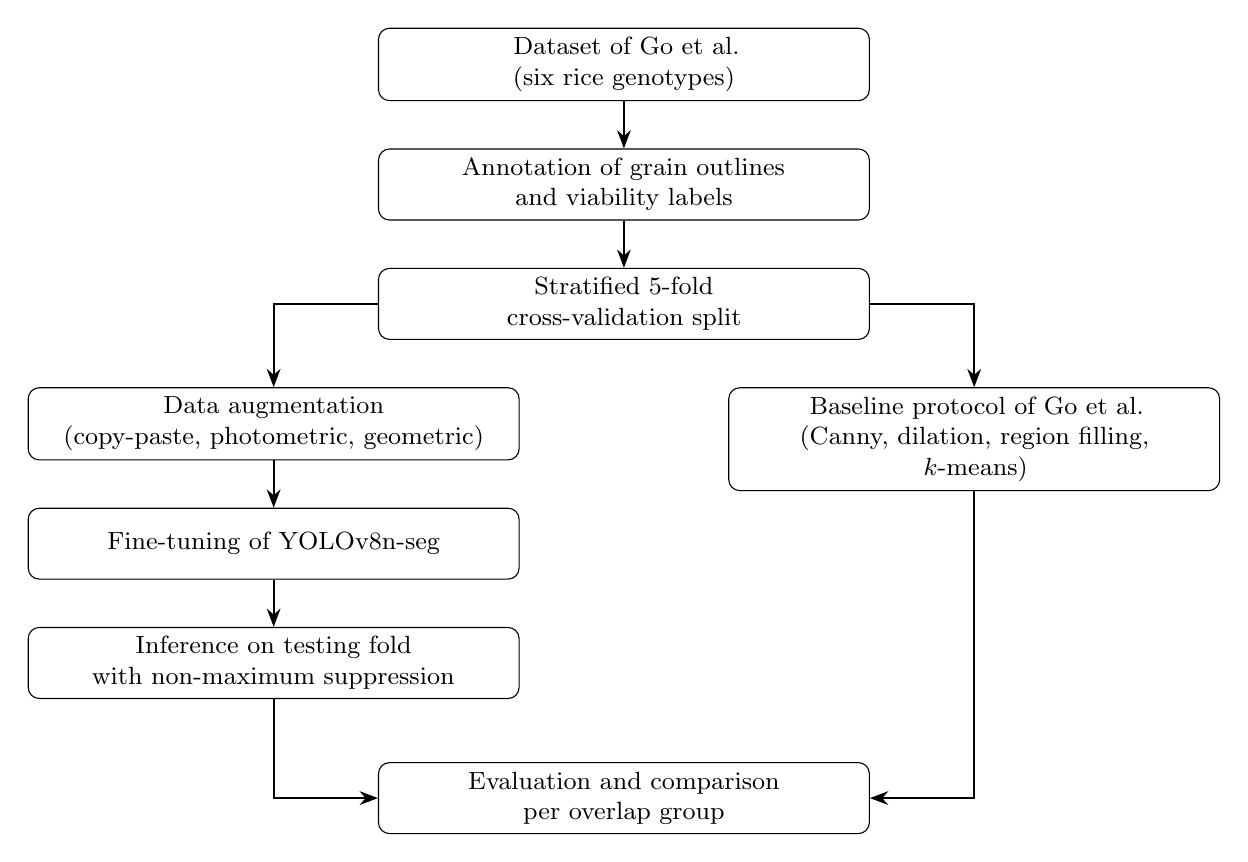
\begin{tikzpicture}[
        node distance=0.6cm and 0.8cm,
        box/.style={draw, rounded corners, align=center, text width=6cm, minimum height=0.9cm, font={\small\hyphenpenalty=10000\relax}},
        side/.style={draw, rounded corners, align=center, text width=6cm, minimum height=0.9cm, font={\small\hyphenpenalty=10000\relax}},
        arrow/.style={-{Stealth}, thick}
    ]
        \node[box] (data) {Dataset of Go et al.\\(six rice genotypes)};
        \node[box, below=of data] (annot) {Annotation of grain outlines\\and viability labels};
        \node[box, below=of annot] (split) {Stratified 5-fold\\cross-validation split};
        \node[side, below left=of split, xshift=2.6cm] (aug) {Data augmentation\\(copy-paste, photometric, geometric)};
        \node[side, below=of aug] (train) {Fine-tuning of YOLOv8n-seg};
        \node[side, below=of train] (infer) {Inference on testing fold\\with non-maximum suppression};
        \node[side, below right=of split, xshift=-2.6cm] (base) {Baseline protocol of Go et al.\\(Canny, dilation, region filling,\\$k$-means)};
        \coordinate (mid) at (infer.south -| split);
        \node[box, below=0.8cm of mid] (eval) {Evaluation and comparison\\per overlap group};

        \draw[arrow] (data) -- (annot);
        \draw[arrow] (annot) -- (split);
        \draw[arrow] (split) -| (aug);
        \draw[arrow] (split) -| (base);
        \draw[arrow] (aug) -- (train);
        \draw[arrow] (train) -- (infer);
        \draw[arrow] (infer) |- (eval);
        \draw[arrow] (base) |- (eval);
    \end{tikzpicture}
    \caption{Overview of the proposed research procedure}
    \label{fig:flowchart}
\end{figure}

\subsubsection{Annotation}
\label{sec:m-annotation}

Each pollen grain in the dataset will be annotated by tracing its outline as a polygon and labeling it as either viable or nonviable using a free annotation tool such as Roboflow or CVAT. Viability labels will follow the same staining criteria used by Go et al.~\cite{go2019}, in which viable and nonviable grains are distinguished by their stain color. In images with lumped pollen, touching or overlapping grains will be traced individually so that each grain is treated as a separate object. The existing grouping of the dataset into images with and without lumped pollen will be retained for evaluation.

\subsubsection{Dataset Preparation}
\label{sec:m-dataset-preparation}

Due to the limited number of images in the dataset, a single training and testing split would leave too few images for reliable evaluation. Therefore, stratified 5-fold cross-validation~\cite{kohavi1995} will be used. The images will be divided into five folds, each containing a proportional number of images with and without lumped pollen, as well as images from each genotype. In each round, one fold will serve as the testing set, while the remaining four folds will be used for training, with 20\% of the training images set aside for validation. This process will be repeated five times so that every image is used for testing exactly once, and the results will be combined across all folds.

To compensate for the small dataset, data augmentation will be applied to the training images only. Copy-paste augmentation~\cite{ghiasi2021} will be used to place annotated pollen grains onto other images so that they overlap, increasing the number of lumped examples. Photometric augmentation, including variations in brightness, contrast, and blur, will account for differences in staining and focus, while geometric augmentation such as flipping and rotation will account for differences in grain orientation. The validation and testing images will not be augmented so that evaluation reflects the original images.

\subsubsection{Model Training}
\label{sec:m-model-training}

Training will be performed using the Ultralytics framework on the free GPU tier of Google Colab. In each fold, the model will be trained with an input size of 640 pixels, a batch size of 8, and a maximum of 50 epochs, using the default optimizer and learning-rate settings of the framework. Mixed-precision training will be used to further reduce memory consumption, and early stopping will end training if the validation performance does not improve for 10 consecutive epochs. The model weights with the best validation performance will then be used for evaluation on the testing fold. Given the small size of the dataset, each training run is expected to take only a few minutes, and all five folds are expected to finish in under an hour.

\subsection{Evaluation and Analysis}
\label{sec:m-evaluation}

\subsubsection{Baseline Method}
\label{sec:m-baseline}

To compare the proposed model with the base study, the image-analysis protocol of Go et al.~\cite{go2019} will be re-implemented using OpenCV, as outlined in Algorithm~\ref{alg:baseline}. Following the original configuration, the pipeline will apply Canny edge detection~\cite{canny1986} with a threshold of 70 to find the boundaries of the pollen grains, dilation with a value of 1 to close small gaps in the detected edges, and region filling to fill the interior of each grain~\cite{gonzalez2018}. The detected grains will then be grouped into two clusters using $k$-means clustering~\cite{lloyd1982} with $k = 2$ on the average grayscale intensity of each grain. Since Go et al.~\cite{go2019} do not state which cluster corresponds to viable pollen, this study assumes that the darker cluster represents viable grains, as viable pollen generally absorbs more stain. This assumption will be checked against the annotations before the baseline is evaluated. Because the baseline does not require training, it will be applied directly to the testing fold of each round so that both methods are compared under identical conditions.

\begin{algorithm}[H]
\caption{Baseline pollen viability identification of Go et al.~\cite{go2019}}
\label{alg:baseline}
\begin{algorithmic}[1]
\Require Microscopic pollen image
\Ensure Viability percentage of the image
\State Apply Canny edge detection with a threshold of 70
\State Apply dilation with a value of 1
\State Apply region filling to obtain each pollen grain
\State Compute the average grayscale intensity of each grain
\State Group the grains into viable and nonviable using $k$-means with $k = 2$
\State Compute the viability percentage using Eq.~\eqref{eq:viability}
\end{algorithmic}
\end{algorithm}

\subsubsection{Performance Metrics}
\label{sec:m-metrics}

The proposed model and the baseline will be evaluated on the testing folds using the metrics summarized in Table~\ref{tab:evaluation}. A predicted grain will be counted as a true positive ($TP$) if it overlaps an annotated grain with an IoU (Eq.~\eqref{eq:iou}) of at least 0.5, following the PASCAL VOC criterion~\cite{everingham2010pascal}, and its predicted viability class matches the annotation. Incorrect predictions are counted as false positives ($FP$), and annotated grains that were not detected are counted as false negatives ($FN$). From these counts, precision, recall, and F1 score~\cite{sokolova2009} will be computed for each class:
\begin{equation}
    \mathrm{Precision} = \frac{TP}{TP + FP}
    \label{eq:precision}
\end{equation}
\begin{equation}
    \mathrm{Recall} = \frac{TP}{TP + FN}
    \label{eq:recall}
\end{equation}
\begin{equation}
    F_1 = 2 \times \frac{\mathrm{Precision} \times \mathrm{Recall}}{\mathrm{Precision} + \mathrm{Recall}}
    \label{eq:f1}
\end{equation}

To allow direct comparison with the 98.3\% and 85.06\% accuracies reported by Go et al.~\cite{go2019}, the accuracy of each image will also be computed for both methods. Since Go et al.~\cite{go2019} do not provide an explicit formula, accuracy will be measured as the agreement between the automated and manual counts of viable and nonviable grains:
\begin{equation}
    \mathrm{Accuracy} = \left(1 - \frac{|\hat{N}_v - N_v| + |\hat{N}_n - N_n|}{N_v + N_n}\right) \times 100
    \label{eq:accuracy}
\end{equation}
where $\hat{N}_v$ and $\hat{N}_n$ are the numbers of viable and nonviable grains counted by the method, and $N_v$ and $N_n$ are the manual counts.

The viability percentage of each image, following Go et al.~\cite{go2019}, is computed as:
\begin{equation}
    V = \frac{N_v}{N_v + N_n} \times 100
    \label{eq:viability}
\end{equation}
where $N_v$ and $N_n$ are the numbers of viable and nonviable grains in the image. The estimated viability percentages will be compared with the manual counts using the mean absolute error (MAE)~\cite{willmott2005}:
\begin{equation}
    \mathrm{MAE} = \frac{1}{n} \sum_{j=1}^{n} \left| \hat{V}_j - V_j \right|
    \label{eq:mae}
\end{equation}
where $n$ is the number of images, $\hat{V}_j$ is the estimated viability percentage, and $V_j$ is the manual viability percentage of image $j$. A lower MAE indicates closer agreement with manual counting. The Pearson correlation coefficient~\cite{pearson1895} will also be computed to measure how consistently the estimated percentages follow the manual counts, where a value closer to 1 indicates stronger agreement.

\subsubsection{Validation and Analysis Procedure}
\label{sec:m-analysis}

All metrics will be computed for both methods and reported separately for images with and without lumped pollen to measure the effect of overlap on performance. Since every image is tested exactly once during cross-validation, the predictions from all five testing folds will be pooled before computing the MAE and Pearson correlation. Following Go et al.~\cite{go2019}, the mean, median, maximum, minimum, and standard deviation of the accuracy across images will be reported for each overlap group. The research objectives will be considered achieved if the proposed model shows a smaller decrease in performance between images without and with lumped pollen than the baseline, and if its viability percentages closely agree with the manual counts. Table~\ref{tab:evaluation} summarizes how each research question will be answered.

\begin{table}[H]
    \centering
    \caption{Evaluation metrics for each research question}
    \label{tab:evaluation}
    \begin{tabular}{p{0.12\linewidth} p{0.38\linewidth} p{0.40\linewidth}}
        \toprule
        \textbf{Question} & \textbf{Purpose} & \textbf{Metrics} \\
        \midrule
        RQ1 & Detection and viability classification & Precision, recall, and F1 score per class \\
        RQ2 & Effect of overlap & Metrics computed separately for images with and without lumped pollen \\
        RQ3 & Comparison with Go et al.~\cite{go2019} & Accuracy, precision, recall, and F1 score of both methods for each overlap group \\
        RQ4 & Agreement with manual counts & MAE and Pearson correlation of viability percentages \\
        \bottomrule
    \end{tabular}
\end{table}


% --------------------------------------------------
% REFERENCES
% --------------------------------------------------

\clearpage
\printbibliography

\end{document}
